\documentclass[a4paper,11pt]{article}
  % Métadonnées
  \title{Exercice sur LaTeX}
  \author{Lecoq Simon (LECS09129600)}
  \date{}

  % Packages
  \usepackage{lmodern,indentfirst}
  \usepackage[font=small,labelfont=bf]{caption}
  \usepackage{tikz,pgfplots}
  \usepackage{multirow,graphbox}
  \usepackage{amsmath,amssymb}
  \usepackage[hyphens]{url}
  \pgfplotsset{compat=1.16}
  \setlength{\parskip}{1em}

  % Corps du document
  \begin{document}

    % TITRE
    \maketitle

    % SECTION I
    \section{Contexte}\label{section:context}
    
      % Sous-section utilisant une image
      \subsection{Présentation de la licence}
      \textit{Pokémon}  est une franchise créée par Satoshi Tajiri en 1996. 
      La marque est gérée partout à travers le monde par la coentreprise \textit{The Pokémon Company}, qui est constitué de \textit{Nintendo}, \textit{Game Freak} et \textit{Creatures}.
      La licence est principalement connue pour les jeux vidéo \textit{Pokémon}, mais elle est également exploitée sous forme de cartes à collectionner, mangas, dessins animés, peluches et autres produits dérivés.
      La mascotte officielle, \textit{Pikachu} (figure \ref{fig:pikachu}), fait désormais partie intégrante de la culture populaire.

      % Image
      \vspace{1em}
      \begin{figure}
        \centering
        
\includegraphics[width=6cm]{images/pikachu.jpg}
        \caption{Illustration de presse de la distribution de \textit{Pikachu} sur \textit{Pokémon Soleil et Lune} pour célébrer les 20 ans de la licence.}
        \label{fig:pikachu}
      \end{figure}

      % Sous-section utilisant des citations (la bibliographie est en fin d'article)
      \subsection{L'impact de \textit{Pokémon} sur la mémoire}
      Si la première génération (1G) des jeux \textit{Pokémon} recense 151 créatures, il y en a désormais plus de 800.
      Dans l'expérimentation de Xie et Zhang \cite{xie_zhang}, deux groupes de participants, l'un ayant joué à la 1G et l'autre n'y ayant jamais joué, doivent déterminer si les \textit{Pokémon} qui leur sont présentés sont déjà apparus dans l'expérimentation ou non.
      Le premier groupe pouvait distinguer plus facilement si c'était le cas lorsque le \textit{Pokémon} provenait de la 1G, tandis que le second groupe n'avait pas spécialement de facilité, montrant ainsi que la mémoire à long terme peut avoir un impact sur la mémoire à court terme.

    % SECTION II
    \section{Mécaniques de jeu}
    Cette section introduit quelques-unes des mécaniques de jeux récurrentes de la série principale des jeux vidéo \textit{Pokémon}.
    Il existe des différences mineures entre les différentes itérations de la série, qui ne sont pas étudiées ici.
    Les informations recueillies proviennent de \textit{Poképedia} \cite{pokepedia}.

      % Sous-section utilisant un schéma Tikz
      \subsection{Niveau}
        Après chaque combat, les \textit{Pokémon} du joueur gagne de l'expérience, ce qui leur permet de monter de niveau afin d'acquérir de nouvelles attaques et de meilleures statistiques de combat.
        En atteignant un certain niveau, il est possible que le \textit{Pokémon} puisse évoluer en un autre \textit{Pokémon}. 
        L'expérience requise pour monter d'un niveau varie de l'espèce, qui est rattachée à l'une des six courbes d'expérience présentes dans le jeu. 
        La figure \ref{fig:exp} illustre trois de ces courbes.

        % Courbes d'expériences
        \vspace{1em}
        \begin{figure}[h]
          \centering
          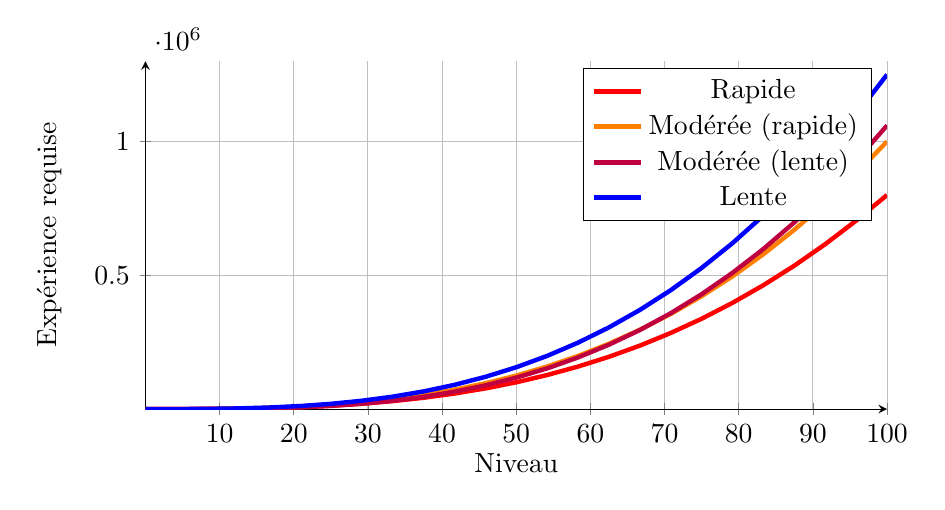
\begin{tikzpicture}
            \begin{axis}[grid=both, xmax=100, ymax=1300000, axis lines=middle, width=11cm, height=6cm, xlabel={Niveau}, x label style={at={(axis description cs:0.5,-0.1)},anchor=north},  ylabel={Expérience requise}, y label style={at={(axis description cs:-0.1,.5)},rotate=90,anchor=south}, every axis plot/.append style={ultra thick}]
              \addplot[red,domain=0:100] {(4*x^3)/5};
              \addlegendentry{Rapide};
              \addplot[orange,domain=0:100] {x^3};
              \addlegendentry{Modérée (rapide)};
              \addplot[purple,domain=0:100] {(6/5)*x^3 - 15*x^2 + 100*x - 140};
              \addlegendentry{Modérée (lente)};
              \addplot[blue,domain=0:100] {(5*x^3)/4};
              \addlegendentry{Lente}
            \end{axis}
          \end{tikzpicture}
          \caption{Expérience requise par niveau.}
          \label{fig:exp}
        \end{figure}

      % Sous-section utilisant un tableau
      \subsection{Table des types}
        L'une des mécaniques de combats dans le jeu \textit{Pokémon} est une variante complexifiée de jeu de \textit{Pierre-Papier-Ciseaux}.
        Chaque \textit{Pokémon} possède jusqu'à deux types (voire trois par l'utilisation d'attaques telles que \textit{Maléfice Sylvain} ou \textit{Halloween}) et chacun de ces types possèdent de multiples faiblesses et résistances.
        La table \ref{table:types} présente quatre des dix-huit types existants.

        % Table des types
        \vspace{1em}
        \begin{table}[h]
          \centering
          \newcommand{\img}[1]{\includegraphics[align=c,scale=1.5]{#1}}
          \begin{tabular}{|p{0.35cm} c|c c c c|}
            \hline
              \multicolumn{2}{|c|}{\multirow{2}{*}{\textbf{VS}}} & \multicolumn{4}{|c|}{\small\textbf{Défenseur}} \\
              & & \img{images/type1.png} & \img{images/type2.png} & \img{images/type3.png} & \img{images/type4.png} \\
            \hline
              \multirow[c]{4}{*}{\rotatebox[origin=c]{90}{\small\textbf{Attaque}}} & \img{images/type1.png} & x0.5 & x0.5 & x2 & x1 \\
              & \img{images/type2.png} & x2 & x0.5 & x0.5 & x1 \\ 
              & \img{images/type3.png} & x0.5 & x2 & x0.5 & x1 \\
              & \img{images/type4.png} & x0.5 & x1 & x2 & x0.5 \\
            \hline
          \end{tabular}
          \caption{Table des types représentant les coefficients multiplicateurs impactant l'efficacité des attaques selon leur type par rapport au type du \textit{Pokémon} défenseur.}
          \label{table:types}
        \end{table}

      % Sous-section utilisant une formule mathématique 
      \subsection{Calcul des dommages}
        L'équation \ref{equation:dmg} est utilisée pour le calcul des dommages lorsqu'un Pokémon en attaque un autre. 
        La valeur $M$ est un multiplicateur qui dépend de nombreux paramètres, tels que le nombre de cibles, la météo, les dégâts critiques (en cas de coup critique), l'efficacité du type (C.f. Table \ref{table:types}) ainsi que le <<Same-Type Attack Bonus>> (octroyé lorsque le type de l'attaquant est identique au type de la compétence utilisée).

        % Equation sur les calcul des dommages
        \begin{equation}
          \label{equation:dmg}
          Dommages = M \times (2 + \frac{(2+\frac{2 \times Niveau}{5}) \times Puissance \times \frac{Attaque}{Defense} }{50})
        \end{equation}

    % REFERENCES
    \begin{thebibliography}{9}
      \bibitem{xie_zhang}
        Xie, W., \& Zhang, W. (2017). Familiarity speeds up visual short-term memory consolidation. Journal of Experimental Psychology: Human Perception and Performance, 43(6), 1207.
      \bibitem{pokepedia}
        Poképedia. (n.d.). Accédé le 02 Décembre, 2018, depuis \url{pokepedia.fr}.
    \end{thebibliography}

  \end{document}